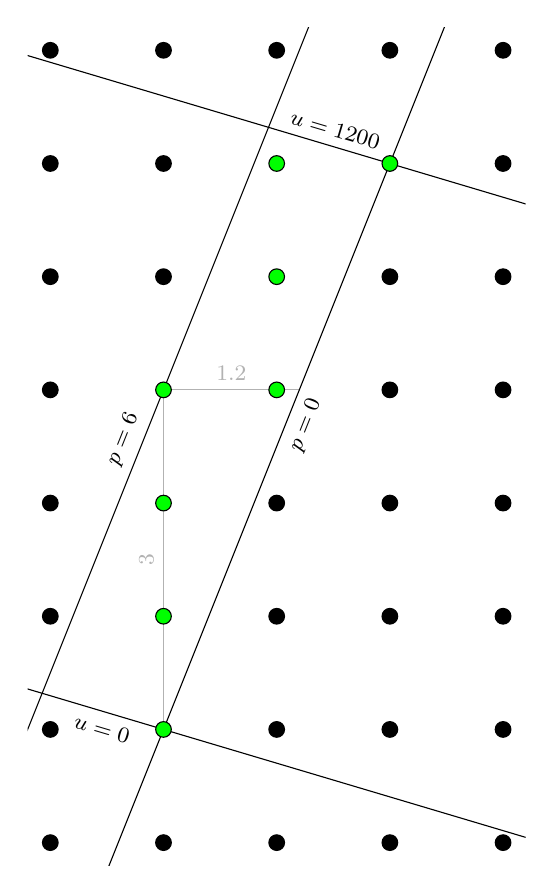
\begin{tikzpicture}[scale=1.4375]

\clip (-1 - 0.2, -1 - 0.2) rectangle (3 + 0.2, 6 + 0.2);

\draw[gray!60] (0, 0) -- (0, 1.5) node[above, rotate=90] {\footnotesize $3$} -- (0, 3);
\draw[gray!60] (0, 3) -- (0.6, 3) node[above] {\footnotesize $1.2$} -- (1.2, 3);

\draw (0 - 2, 0 - 5) -- (0 + 0.55 * 2, 0 + 0.55 * 5) node[below, rotate=68.2] {\footnotesize $p=0$} -- (0 + 2 * 2, 0 + 2 * 5);
\draw (0 - 2, 3 - 5) -- (0 - 0.1 * 2, 3 - 0.1 * 5) node[above, rotate=68.2] {\footnotesize $p=6$} -- (0 + 2 * 2, 3 + 2 * 5);

\draw (-2, -2 * -63.90/214.44) -- (-0.5, -0.5 * -63.90/214.44) node[below, rotate=-16.59] {\footnotesize $u=0$} -- (7, 7 * -63.90/214.44);
\draw
    (-2, -2 * -63.90/214.44 + 1200/214.44) --
    (1.475, 1.475 * -63.90/214.44 + 1200/214.44) node[above, rotate=-16.59] {\footnotesize $u=1200$} --
    (7, 7 * -63.90/214.44 + 1200/214.44);
\draw (-1, -1) node[circle,draw=black,fill=black,inner sep=2pt] {};
\draw (-1, 0) node[circle,draw=black,fill=black,inner sep=2pt] {};
\draw (-1, 1) node[circle,draw=black,fill=black,inner sep=2pt] {};
\draw (-1, 2) node[circle,draw=black,fill=black,inner sep=2pt] {};
\draw (-1, 3) node[circle,draw=black,fill=black,inner sep=2pt] {};
\draw (-1, 4) node[circle,draw=black,fill=black,inner sep=2pt] {};
\draw (-1, 5) node[circle,draw=black,fill=black,inner sep=2pt] {};
\draw (-1, 6) node[circle,draw=black,fill=black,inner sep=2pt] {};
\draw (0, -1) node[circle,draw=black,fill=black,inner sep=2pt] {};
\draw (0, 0) node[circle,draw=black,fill=green,inner sep=2pt] {};
\draw (0, 1) node[circle,draw=black,fill=green,inner sep=2pt] {};
\draw (0, 2) node[circle,draw=black,fill=green,inner sep=2pt] {};
\draw (0, 3) node[circle,draw=black,fill=green,inner sep=2pt] {};
\draw (0, 4) node[circle,draw=black,fill=black,inner sep=2pt] {};
\draw (0, 5) node[circle,draw=black,fill=black,inner sep=2pt] {};
\draw (0, 6) node[circle,draw=black,fill=black,inner sep=2pt] {};
\draw (1, -1) node[circle,draw=black,fill=black,inner sep=2pt] {};
\draw (1, 0) node[circle,draw=black,fill=black,inner sep=2pt] {};
\draw (1, 1) node[circle,draw=black,fill=black,inner sep=2pt] {};
\draw (1, 2) node[circle,draw=black,fill=black,inner sep=2pt] {};
\draw (1, 3) node[circle,draw=black,fill=green,inner sep=2pt] {};
\draw (1, 4) node[circle,draw=black,fill=green,inner sep=2pt] {};
\draw (1, 5) node[circle,draw=black,fill=green,inner sep=2pt] {};
\draw (1, 6) node[circle,draw=black,fill=black,inner sep=2pt] {};
\draw (2, -1) node[circle,draw=black,fill=black,inner sep=2pt] {};
\draw (2, 0) node[circle,draw=black,fill=black,inner sep=2pt] {};
\draw (2, 1) node[circle,draw=black,fill=black,inner sep=2pt] {};
\draw (2, 2) node[circle,draw=black,fill=black,inner sep=2pt] {};
\draw (2, 3) node[circle,draw=black,fill=black,inner sep=2pt] {};
\draw (2, 4) node[circle,draw=black,fill=black,inner sep=2pt] {};
\draw (2, 5) node[circle,draw=black,fill=green,inner sep=2pt] {};
\draw (2, 6) node[circle,draw=black,fill=black,inner sep=2pt] {};
\draw (3, -1) node[circle,draw=black,fill=black,inner sep=2pt] {};
\draw (3, 0) node[circle,draw=black,fill=black,inner sep=2pt] {};
\draw (3, 1) node[circle,draw=black,fill=black,inner sep=2pt] {};
\draw (3, 2) node[circle,draw=black,fill=black,inner sep=2pt] {};
\draw (3, 3) node[circle,draw=black,fill=black,inner sep=2pt] {};
\draw (3, 4) node[circle,draw=black,fill=black,inner sep=2pt] {};
\draw (3, 5) node[circle,draw=black,fill=black,inner sep=2pt] {};
\draw (3, 6) node[circle,draw=black,fill=black,inner sep=2pt] {};
\end{tikzpicture}
